\chapter{Results}\label{chp:results}

What happens in this chapter?

Recapitulate the predictions for reaction times
\section{Descriptive Statistics} \label{sec:desc_stats}

Present means and boxplots, discuss in regards to the above predictions
Possibly include a t-tests as a foretaste
\begin{figure}[h]
    \centering
    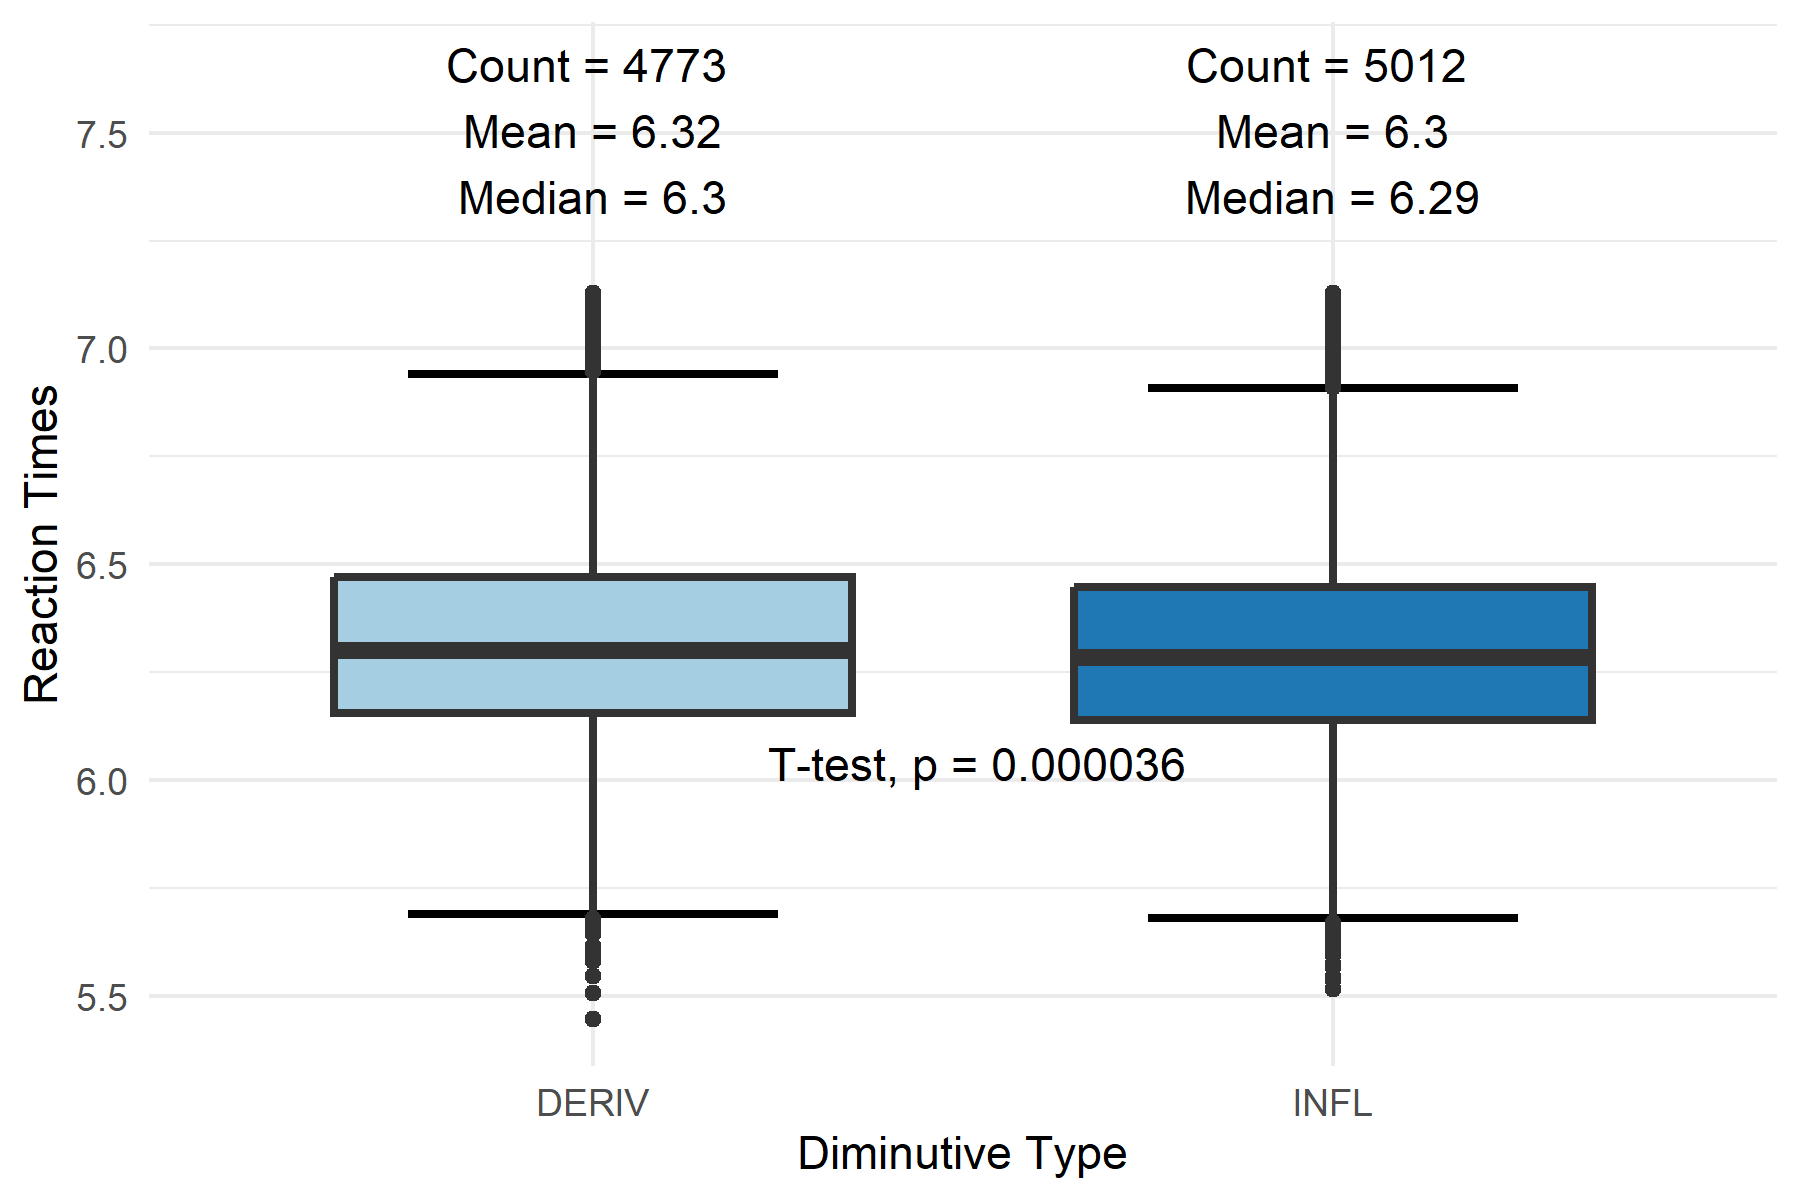
\includegraphics[width=\textwidth]{images/dim_box.png}
    \caption{Boxplot of Diminutive Type}
    \label{fig:boxplot}
\end{figure}

\section{Inferential Statistics} \label{sec:inf_stats}
\begin{itemize}
\item Present the final model formula
\end{itemize}

\begin{table}[h]
\centering
\label{tab:regressionrt}
\resizebox{0.8\textwidth}{!}{%
\begin{tabular}{lccc}
\toprule
\textbf{Predictor} & \textbf{Estimate} & \textbf{SE} & \textbf{\textit{p}-Value}  \\ \midrule
(Intercept) & 6.3137 & 0.0161 & \textbf{>0.001}\\
Diminutive Type & -0.0032 & 0.0036 & 0.3669 \\
Frequency  & -0.0245 & 0.0045 & \textbf{>0.001} \\
Morpheme Count & 0.0026 & 0.0051 & 0.6089 \\
Orth. Neighbourhood & 0.0202 & 0.0052 & \textbf{>0.001} \\
Concreteness & 0.0020 & 0.0038 & 0.5962 \\
Age of Acquisition & 0.0168 & 0.0043 & \textbf{>0.001} \\
Word Prevalence & -0.0471 & 0.0085 & \textbf{>0.001} \\
Dim. Type*Frequency & 0.0071 & 0.0032 & \textbf{0.0298} \\
\bottomrule
\end{tabular}%
}
\caption{Summary of fixed effects.}
\end{table}

\subsection{Diminutive Type} \label{subsec:dimtype}
The predictions for diminutive type are replicated in the model, as there is an observable predicted change in estimate depending on the type of diminutive. While derived wordforms are predicted to require less time to recognise, the predictor is not statistically significant on its own, while its effect size is miniscule. However, due to the presence of an interaction term in the model, the effect of diminutive type is not interpretable on its own; diminutive type and frequency are conditioned on each other, and their effects need to be interpreted together \parencite{Winter+2019}. See Subsection \ref{subsec:interaction} below for an interpretation of the interaction.
\subsection{Frequency} \label{subsec:freq}
Frequency is historically one of the most robust predictors in lexical recognition studies \parencite{Brysbaert+etal+2016}. Higher surface frequency is consistently associated with lower reaction times, as more frequently used words are postulated to require less time for lexical activation. These particular frequency values are based on an expanded version of the subtitle corpus SUBTLEX-NL \parencite{Keuleers+etal+2010}. In addition, the values have been Zipf-transformed to arrive at a standardized frequency measure independent of corpus size \parencite{vanHeuven+etal+2014}. Higher Zipf values reflect higher word frequencies and are therefore predicted to elicit lower reaction times. This prediction holds up in our model, with Zipf-tansformed frequency being a facilitating factor with one of the largest effect sizes in the whole model. Again, because of the interaction term, the effect of frequency cannot be interpreted independently from diminutive type.
\subsection{Morpheme Count} \label{subsec:nmorph}
The number of morphemes is an approximate measurement for a wordform's internal complexity. While the values assigned to each wordform are theory-specific, the general prediction under the assumption of full decomposition is the same: more internally complex words require longer to decompose into constituent morphemes, look those morphemes up, recombine them into the wordform in question, and check for well-formedness. This prediction is upheld in the model above; however, while the variable is predicted to be inhibitory, the effect size is rather negligible, and the predictor does not make a statistically significant contribution to the model.
\subsection{Orthographic Neighbourhood} \label{subsec:old20}
Orthographic neighbourhood is a measure of how similar a word is to its immediate orthographic neighbours as determined by a set inventory of possible permutations such as letter substitution and/or transposition, addition or subtraction. While there exist multiple ways of quantifying neighbourhood effects, the one chosen for this analysis is the orthographic Levenshtein distance based on the closest 20 words (OLD20, \cite{Yarkoni+etal+2008}). Higher OLD20 ratings reflect the average number of permutations needed to transform a wordform into one of its 20 closest neighbours, and the higher the rating, the less similar the wordform is to its neighbours. The attested effect of OLD20 is therefore inhibitory \parencite[among others]{Brysbaert+etal+2016}, as more dissimilar items take longer to recognize. The model above replicates the prediction: OLD20 is a statistically significant predictor with a sizeable inhibitory effect.
\subsection{Concreteness} \label{subsec:concreteness}
A predictor adopted from \cite{Brysbaert+etal+2014}, concreteness quantifies the degree to which a given wordform refers to a perceivable entity, e.g. a object in the real world compared to an abstract concept. It is represented on a 5-point scale and based on averaged subjective ratings collected from 75 students at the University of Leuven. According to \cite{Brysbaert+etal+2014}, more concrete words are predicted to require less time to recognize. However, \cite{Brysbaert+etal+2016} report a reverse effect of concreteness, with less concrete words predicting lower reaction times. They attempt to explain this inversion through the typically higher emotional load of more abstract wordforms compared to their more concrete counterparts: strongly positive or negative wordforms induce quicker responses. While the model above reflects the inverted prediction as reported in \cite{Brysbaert+etal+2016}, the predictor is not statistically significant, while its effect size is the lowest in the entire model.
\subsection{Age of Acquisition} \label{subsec:aoa}
Another predictor based on subjective ratings from students is the age of acquisition (AoA), similarly adopted from \cite{Brysbaert+etal+2014}. Despite the name, it does not reflect the actual average age when the wordform is acquired, and functions instead as an estimate of processing cost: in the process of value assignment, a word is given an age of acquisition rating based on how (self-reportedly) easy it is to understand it, the rationale being something like "this is an easy word; thus, I must have learned it early" \parencite[p.23]{Brysbaert+etal+2016}. Higher AoA values therefore predict longer reaction times and are replicated as such in the model: the predictor is statistically significant and its effect size is relatively substantial.
\subsection{Word Prevalence} \label{subsec:prevalence}
A novel explanatory variable proposed by \cite{Keuleers+etal+2015} and introduced in the Dutch Lexicon Project 2 dataset, word prevalence is defined as "word knowledge in the population" \parencite{Brysbaert+etal+2016} and intended as a supplementary predictor to word frequency. Frequency is corpus-dependent and is not always the most reliable measure of how well-known or widely-used a wordform is: for example, words referring to household objects are well-known in the general population, but this fact is not represented in their (typically low) frequency scores. Word prevalence was introduced to account for this as well as other predictive shortcomings of frequency. Its prediction is straightforward: the better-known a word, the less time it takes to recognise. The values for prevalence were collected by \cite{Keuleers+etal+2015} from over 100.000 Dutch-speaking participants from Flanders. Both \cite{Keuleers+etal+2015} and \cite{Brysbaert+etal+2016} report the predictor as one of the most correlated with reaction times, usually second-best after (and in some cases even more explanatory than) frequency. As such, it is no surprise to see this effect replicated in a model based on a subset of the DLP2: word prevalence is a facilitatory explanatory variable with the single largest effect size in the entire model.
\subsection{Interaction of Diminutive Type and Frequency} \label{subsec:interaction}
hehe
\subsection{Random Effects}
hehe

\section{Summary} \label{sec:stats_summary}
\begin{itemize}
\item Sum up all facts, no opinion on the facts
\end{itemize}
